\documentclass{gescons}

\genre {Entrevista}
\author{Helena Araújo}
\title{Libertações Evolutivas: Trajetórias Semperaprendente sob Olhar Conscienciológico}


\begin{document}
    \makeentrevistatitle
    \coverart{back/Helena_Araujo}

    \begin{multicols}{2}

\begin{center}
    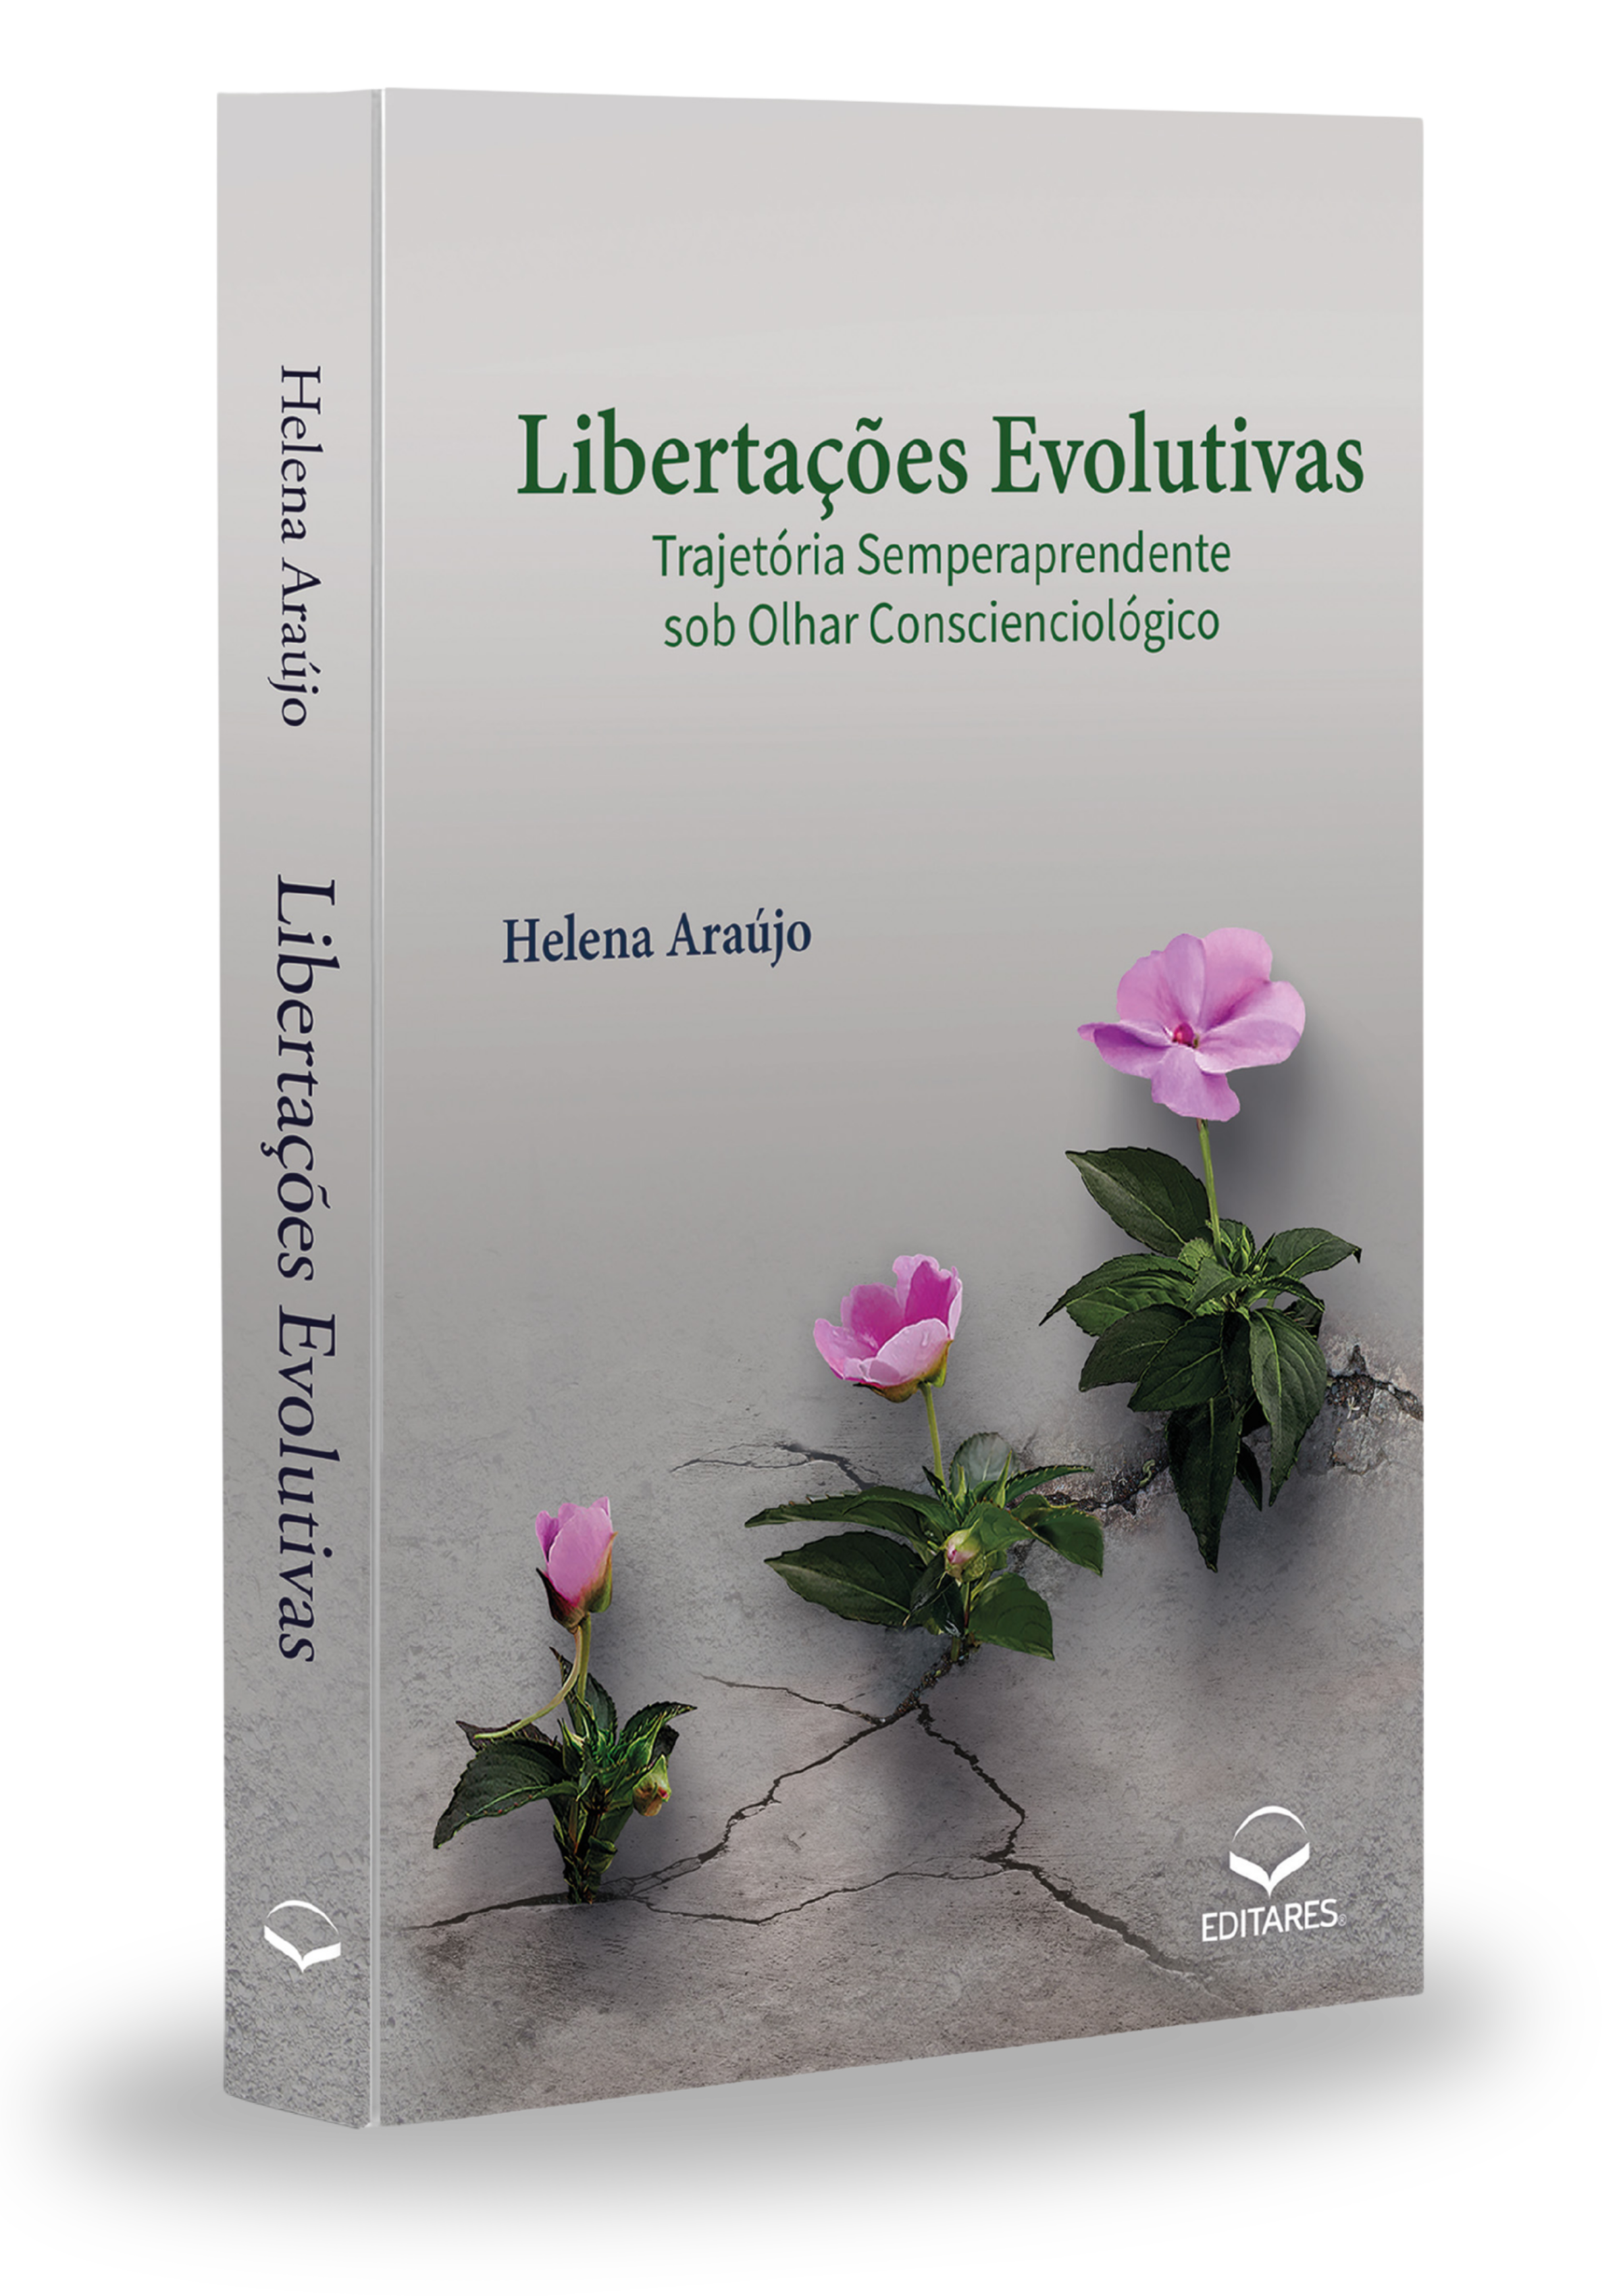
\includegraphics[width=6cm]{articles/entrevista/mockups/Helena_Araujo.png}
\end{center}


\subsubsection{1. Qual foi a motivação para a escrita da obra? Por que a definição deste tema para publicação de um livro?}

A imagem da capa traduz a motivação para a escrita do livro. Encontrei, na rachadura de um cimento, a linda planta \emph{vinca}, bem verde e com flor. Naquele momento, fiz a associação de que as adversidades enfrentadas na minha vida foram muito duras, mas com esforço, antivitimização e amparo sempre encontrei uma ``brecha'' para libertar-me. As vivências conscienciológicas possibilitaram-me a reciclagem intraconsciencial vendo nas crises oportunidades evolutivas. Por esse motivo escrevi minha trajetória semperaprendente com o propósito de compartilhar o que aprendi com as pessoas interessadas na compreensão de si mesmo e do outro.

\begin{pullquote}
``As vivências conscienciológicas possibilitaram-me a reciclagem intraconsciencial vendo nas crises oportunidades evolutivas.''
\end{pullquote}

\subsubsection{2. Quais foram as principais percepções, intra e extrafísicas, durante a pesquisa e a escrita da obra? E posterior ao lançamento?}

Este livro é resultado do laboratório consciencial desenvolvido mediante a análise da infância, adolescência, juventude e adultidade; da maxidissidência religiosa; dos enfrentamentos e autossuperações. Tive a sensação de empreender longa viagem em busca de mim mesma. A escrita da obra ampliou sobremaneira a autopesquisa possibilitando a desdramatização da morte no grupo familiar, os acertos grupocármicos a partir de retrocognições; assistência a mães que perderam filhos na guerra; reurbanização extrafísica de ambiente degradado.


\subsubsection{3. Qual o maior aprendizado com a escrita desta obra?}


O acesso ao Paradigma consciencial foi avanço significativo para a aceleração da história pessoal. A publicação do livro \emph{Libertações Evolutivas: Trajetórias Semperaprendente sob Olhar Conscienciológico} possibilitou ressignificar o jeito de ser e agir; estender novo olhar sobre os emaranhamentos da vida, entender melhor as pessoas e os acontecimentos. Os problemas continuaram surgindo tanto individuais quanto no grupocarma. O que mudou foi a forma de lidar com eles. Isso resultou nas minhas libertações evolutivas. \emph{Considero ter vivido o ocaso desta existência um feliz entardecer.}

\subsubsection{4. O que poderia dizer como incentivo para que mais pesquisadores invistam na publicação de obras conscienciológicas?}

Aos futuros autores, gostaria de dizer que o exame autobiográfico é excelente tema para a autopesquisa, pois ajuda a perceber o que é preciso reciclar. Escrever o livro é também começar parceria afetiva consigo mesmo que resulte em autoestima, alegria de viver, bom humor, equilíbrio holos­somático e melhor convívio com todos, expandindo este processo para a assis­tência lúcida com base na maxifraternidade.


\begin{pullquote}
``Com a escrita de um livro, o autor pode conquistar novas posturas, hábitos, intenções e   alicerçar melhores escolhas para esta e outras vidas futuras.''
\end{pullquote}
    
    \end{multicols}
\end{document}
